\documentclass[border=6pt]{standalone}
\usepackage{amsmath}
\usepackage{tikz}
\usepackage{pgfplots}
\pgfplotsset{compat=1.18}
\usetikzlibrary{arrows.meta,calc,positioning}

% Draw one thermometer: a uniform tube+bulb container, with tick marks
% placed at computed y-positions so that the reference tick sits at y=0
% (local scope), letting a single global horizontal line cross all three
% thermometers at their aligned reference reading.
% #1 = x shift (cm), #2 = title, #3 = list of (value,y,label-or-empty) tuples
\newcommand{\thermometer}[3]{%
  \begin{scope}[xshift=#1 cm]
    % title
    \node[align=center, font=\bfseries\small] at (0,4.3) {#2};
    % tube
    \draw[thick, rounded corners=6pt, fill=white] (-0.5,-2.6) rectangle (0.5,3.7);
    % bulb
    \draw[thick, fill=white] (0,-3.1) circle (0.55);
    % connector so bulb visually joins tube
    \draw[thick, fill=white] (-0.5,-2.9) rectangle (0.5,-2.6);
    #3
  \end{scope}
}

\begin{document}
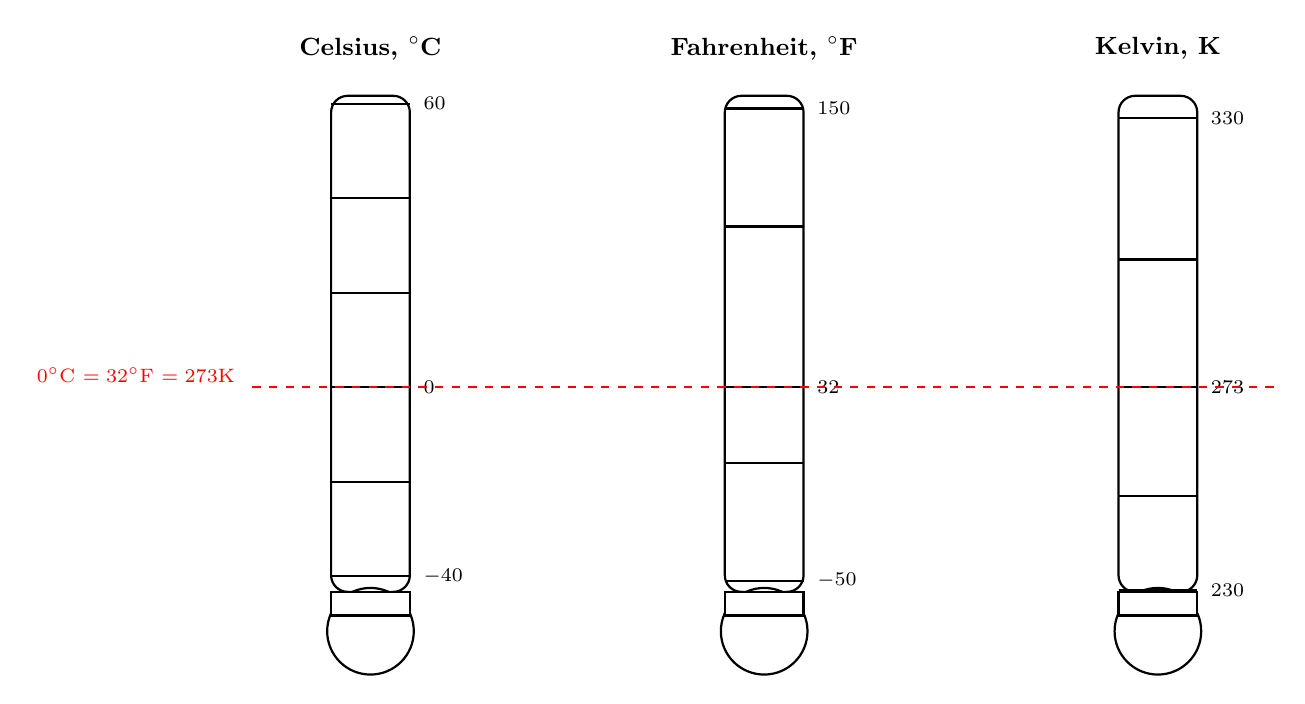
\begin{tikzpicture}[
    tick/.style={thick},
    lbl/.style={font=\scriptsize, anchor=west},
]

% ---------- Celsius: range -40 to 60, k=0.06 cm/deg, ref 0C at y=0 ----------
\thermometer{0}{Celsius, $^\circ$C}{
  \draw[tick] (-0.5,-2.4) -- (0.5,-2.4); \node[lbl] at (0.55,-2.4) {$-40$};
  \draw[tick] (-0.5,-1.2) -- (0.5,-1.2);
  \draw[tick] (-0.5,0)    -- (0.5,0);    \node[lbl] at (0.55,0)    {$0$};
  \draw[tick] (-0.5,1.2)  -- (0.5,1.2);
  \draw[tick] (-0.5,2.4)  -- (0.5,2.4);
  \draw[tick] (-0.5,3.6)  -- (0.5,3.6);  \node[lbl] at (0.55,3.6) {$60$};
}

% ---------- Fahrenheit: range -50 to 150, k=0.03 cm/deg, ref 32F at y=0 ----------
\thermometer{5}{Fahrenheit, $^\circ$F}{
  \draw[tick] (-0.5,-2.46) -- (0.5,-2.46); \node[lbl] at (0.55,-2.46) {$-50$};
  \draw[tick] (-0.5,-0.96) -- (0.5,-0.96);
  \draw[tick] (-0.5,0)     -- (0.5,0);     \node[lbl] at (0.55,0)     {$32$};
  \draw[tick] (-0.5,2.04)  -- (0.5,2.04);
  \draw[tick] (-0.5,3.54)  -- (0.5,3.54);  \node[lbl] at (0.55,3.54) {$150$};
}

% ---------- Kelvin: range 230 to 330, k=0.06 cm/deg, ref 273K at y=0 ----------
\thermometer{10}{Kelvin, K}{
  \draw[tick] (-0.5,-2.58) -- (0.5,-2.58); \node[lbl] at (0.55,-2.58) {$230$};
  \draw[tick] (-0.5,-1.38) -- (0.5,-1.38);
  \draw[tick] (-0.5,0)     -- (0.5,0);     \node[lbl] at (0.55,0)     {$273$};
  \draw[tick] (-0.5,1.62)  -- (0.5,1.62);
  \draw[tick] (-0.5,3.42)  -- (0.5,3.42);  \node[lbl] at (0.55,3.42) {$330$};
}

% Reference line: 0C = 32F = 273K, all aligned at local y = 0
\draw[red, dashed, thick] (-1.5,0) -- (11.5,0);
\node[red, font=\scriptsize, anchor=east] at (-1.6,0.15) {$0^\circ$C $=32^\circ$F $=273$K};

\end{tikzpicture}
\end{document}
